\chapter{Methodology}

%%%%%%%%%%%%%%%%%%%%%%%%%%%%%%%%%%%%%%%%%%%%%%%%%%%%%%%%%%%%%%%

\begin{figure}
\centering
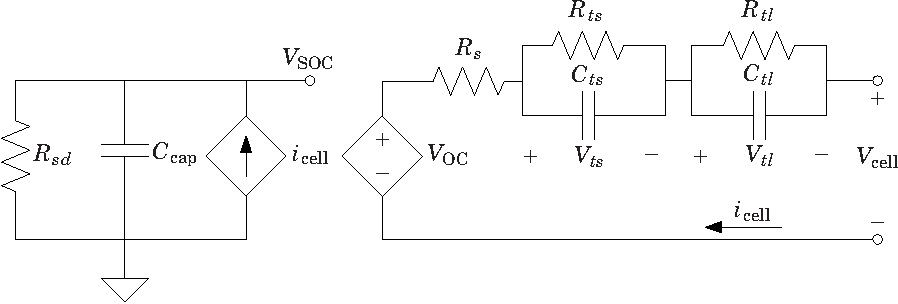
\includegraphics[width=0.9\textwidth]{batt_model}
\caption{Battery model for simulation. [This is taken from a paper, but I will probably redo it and change some labels, e.g. Rseries to Rs]}
\label{fig:batt_model}
\end{figure}

The nonlinear parameters of the model for a typical lithium-ion battery are [need source]
\begin{align}
	R_s &= 0.1562 e^{-24.37 V_{SOC}} + 0.07446 \\
	R_{ts} &= 0.3208 e^{-29.14 V_{SOC}} + 0.04669 \\
	C_{ts} &= -752.9 e^{-13.51 V_{SOC}} + 703.6 \\
	R_{tl} &= 6.603 e^{-155.2 V_{SOC}} + 0.04984 \\
	C_{tl} &= -6056 e^{-27.12 V_{SOC}} + 4475 \\
	V_{OC} &= -1.031 e^{-35 V_{SOC}} + 3.685 + 0.2156 V_{SOC} - 0.1178 V_{SOC}^2 + 0.3201 V_{SOC}^3
\end{align}
The circuit on the left is a linear, time-invariant (LTI) system, which has the following state space model:
\begin{gather}
    x = C_\text{cap} V_{SOC} \\
    \dot{x} = \frac{x}{R_{sd} C_\text{cap}} - \frac{i_\text{cell}}{C_\text{cap}} \\
    V_{SOC} = \frac{x}{C_\text{cap}}
\end{gather}
The circuit on the right is a nonlinear system, since the coefficients are dependent on the voltage $V_{SOC}$. The corresponding state space model is [I think that I changed the model a little for my simulations by adding an output for $i_\text{cell}$. Also, the ``nonlinear'' simulations combine both ss systems using the given Voc nonlinearity].
\begin{gather}
	\dot{x} = \begin{bmatrix}
		-1/R_{ts}C_{ts} & 0 & 0 \\
		0 & -1/R_{tl}C_{tl} & 0 \\
		0 & 0 & 0
		\end{bmatrix} x 
		+ \begin{bmatrix} 1/C_{ts} & 1/C_{tl} \end{bmatrix} i_\text{cell} \\
	v_\text{cell} = [-1 \quad -1 \quad 1] x - R_s i_\text{cell}
\end{gather}

\begin{figure}
\centering
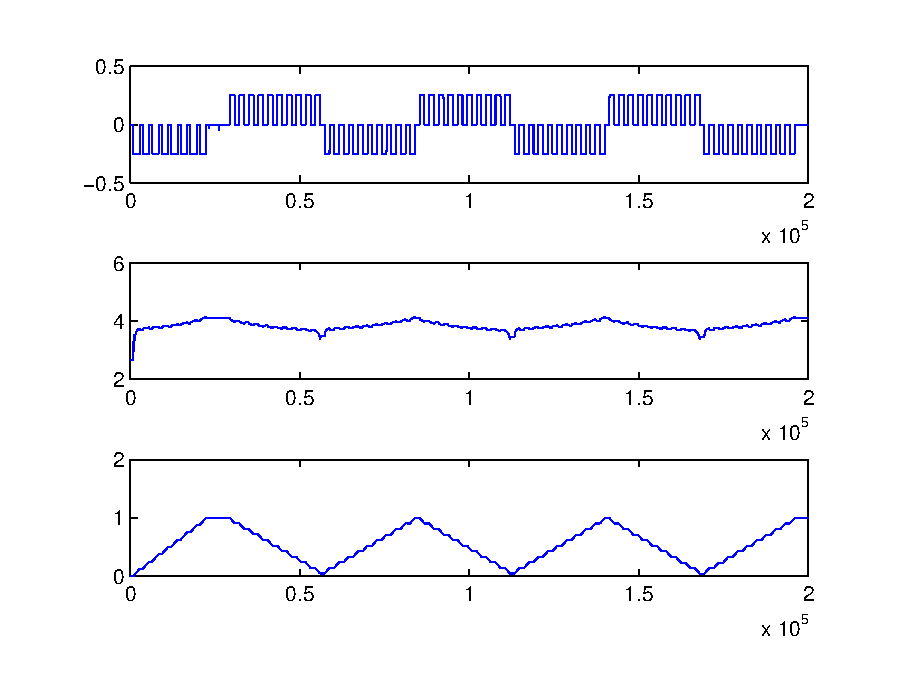
\includegraphics[width=0.9\textwidth]{sim_ideal}
\caption{Discharge current along with the resulting voltage and SOC.}
\label{fig:idealsim}
\end{figure}
